\documentclass{article} % For LaTeX2e
\usepackage{nips15submit_e,times}
\usepackage{hyperref}
\usepackage{graphicx}
\usepackage{url}



\title{Preliminary Result for Hessian-Free Optimization and Text Prediction with RNN}


\author{
Joseph Bybee\\
University of Michigan\\
\texttt{} \\
\and
Byoungwook Jang\\
University of Michigan \\
Address \\
\texttt{bwjang@umich.edu} \\
}


\newcommand{\fix}{\marginpar{FIX}}
\newcommand{\new}{\marginpar{NEW}}

%\nipsfinalcopy % Uncomment for camera-ready version

\begin{document}

\maketitle

\begin{abstract}
The problem of text prediction is a popular area of study within the machine learning community. The problem involves training an agent that observes a sequence of words and predicts the next word in the sequence. More formally, this problem can be understood as a language modeling problem where we want to form some probability distribution for a word $w_t$ in period $t$ based on the observed corpus of words for the previous periods $w_{t-1}$. Our project implements recurrent neural networks (RNNs) to solve this text prediction problem and focuses on different optimization methods to train RNNs and their performances. These methods include hessian-free optimization with a damping scheme, stochastic gradient descent, and Long Short-Term Memory (LSTM).
\end{abstract}

\section{Word Corpus Data}
Natural Language Toolkit (NLTK) provides a variety of text data that can be used to test our RNNs. It provides lexical resources such as WordNet as well as text processing libraries for classification, tokenization, tagging, and parsing that would allow us to easily train and test RNNs [1]. As a part of the preliminary work, we focused on experimenting with NLTK library to tokenize a given text data, where we used the Brown Corpus as a starting point.  We plan to train our RNNs on different kinds of text and look into what kinds of sentences are generated based on the training corpus.

\section{Hessian-Free Method}
The implementation of RNNs using different optimization in this project is largely based on Marten's paper [2]. The Hessian-free optimization method used in this work was adopted from Marten's optimization for Deep learning [3]. The implementation of Hessian-free method in our project was adopted from Boulanger-Lewandowski's software, which utilizes Theano library from Python to build a general purpose optimization for RNNs in Theano [4]. 

Our preliminary results focus on understanding Theano library and adopting Boulanger's implementation to optimize RNNs for our problem of text prediction using the Hessian-free method. Once we validate this adoption of Theano library based Hessian optimization, the rest of the project will involve implementing stochastic gradient descent and LSTM to train RNNs and comparing the performances. Once the empirical comparisons are completed, more in depth analysis of Gauss-Newton matrix and its role in the Hessian-free method will be provided in our final report.

\newpage

\section{Preliminary result for Hessian-Free Method}

To test our code, we generated a sample dataset and used softmax functions for the classification layer. Our sample dataset include 5 input variables, 3 classes of output and 1000 samples.  The 3 classes were generated using soft thresholding based on the input vectors. Our model went through 100 100 updates to get an estimation. Figure \ref{fig:error} shows a plot of the number of errors for each update. Each update continues to improve the performance of the new model. 

The data generating process and the model fit is also demonstrated in figure \ref{fig:structure}.  The first portion of this figure shows the value for each of the input elements, while the second part shows the model fit.  The blue line shows the true value while the gray scale portion shows the probability estimated by the model. We plan to experiment with the sample output result and look at the number of incorret tokens tagged by our trained RNNs. Working on this next step will allow us to create a probability distribution of each word based on their tokens, and thus gives our model better context to solve the text prediciton task.

\begin{figure}
\centering
\caption{Errors}
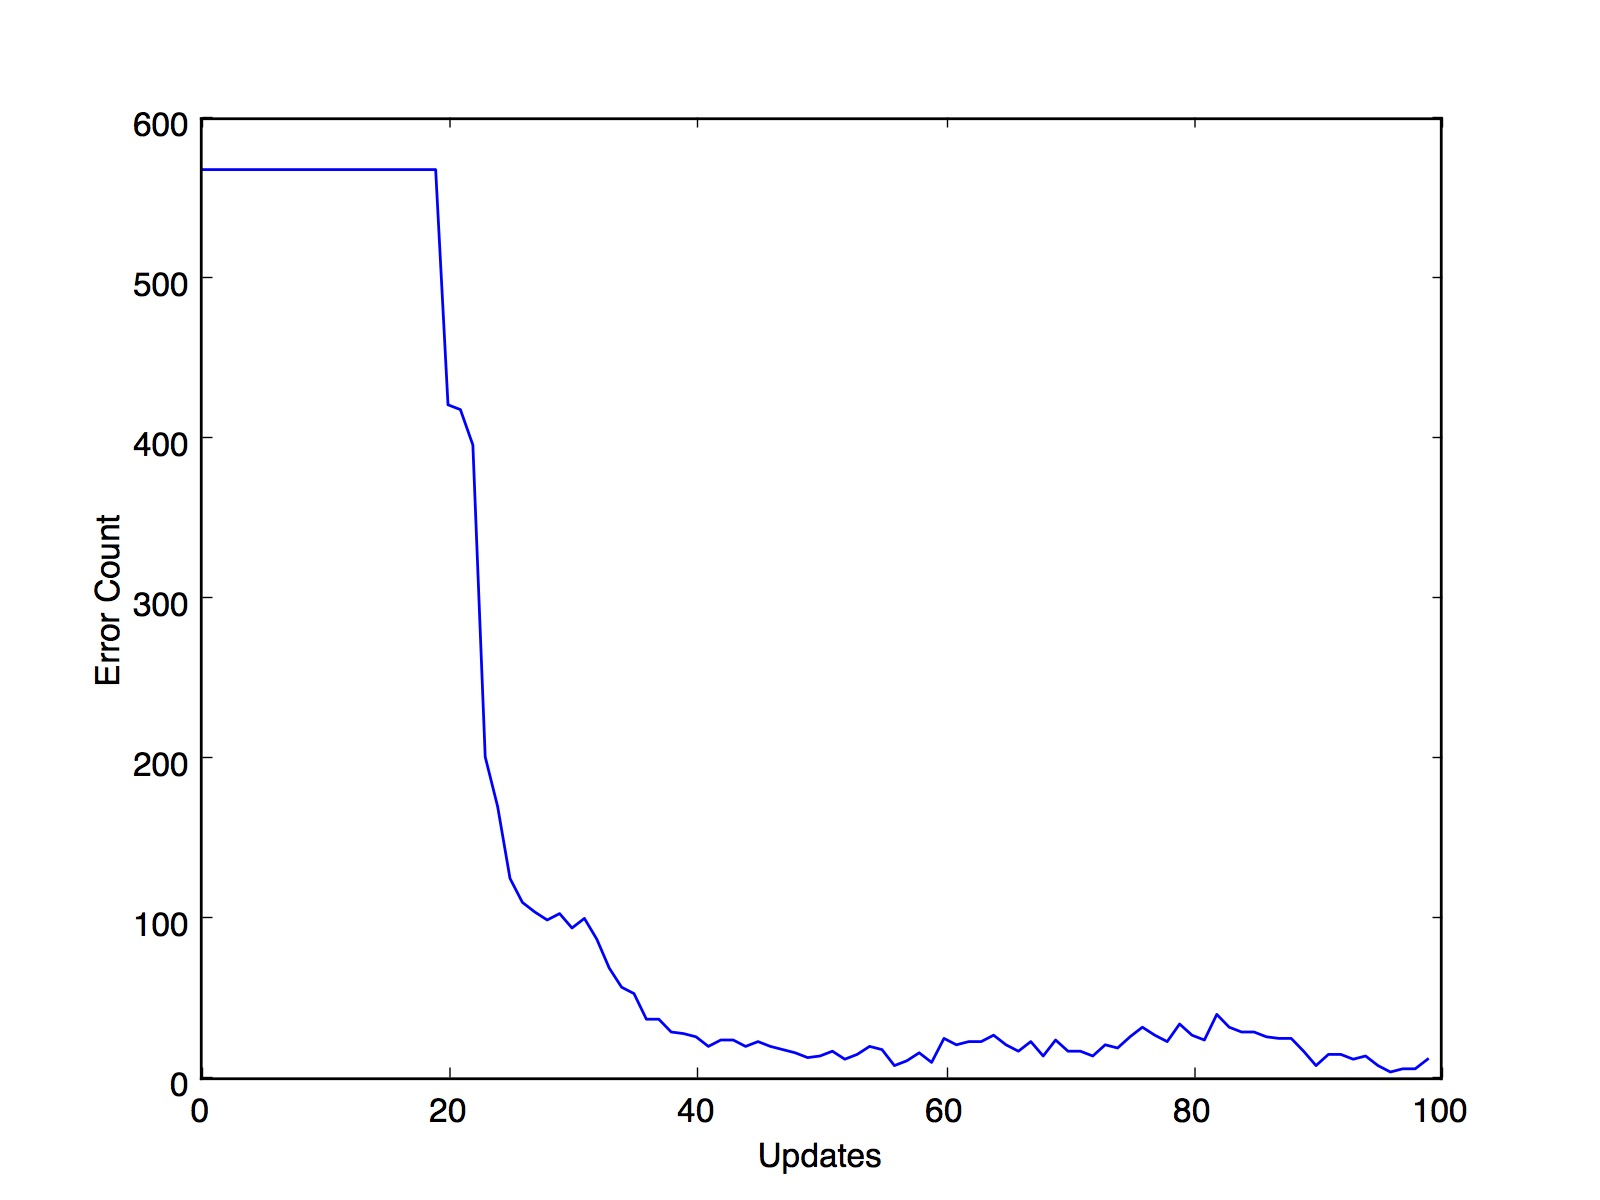
\includegraphics[width=0.5\linewidth]{errors.jpg}
\label{fig:error}
\end{figure}

\begin{figure}
\centering
\caption{Model Structure}
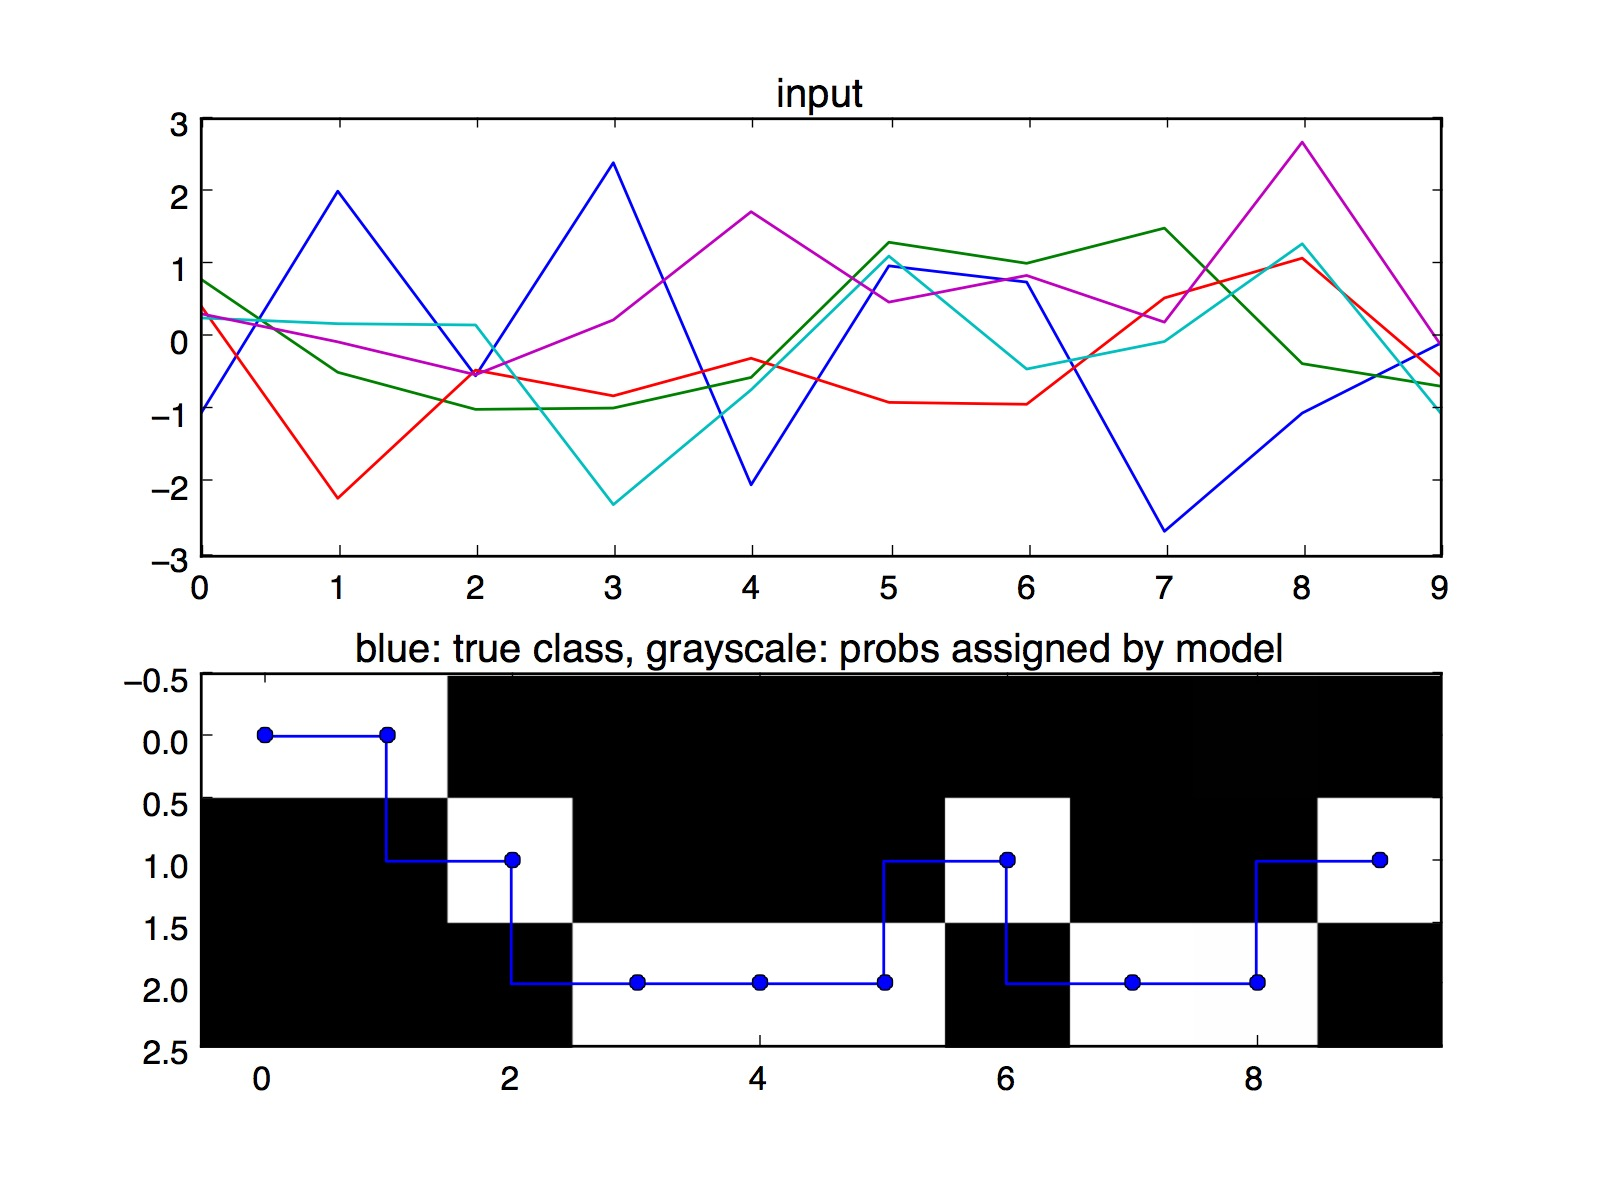
\includegraphics[width=0.5\linewidth]{results.jpg}
\label{fig:structure}
\end{figure}

\subsubsection*{References}


\small{
[1] S. Bird, E. Loper and E. Klein (2009), Natural Language Processing with Python. O?Reilly Media Inc.

[2] J. Martens, and I. Sutskever (2011), Learning Recurrent Neural Networks with Hessian-Free Optimization. In Proceedings of the 28th International Conference on Machine Learning (ICML).

[3] J. Martens (2010), Deep Learning via Hessian-free Optimization, In Proceedings of the 27th International Conference on Machine Learning (ICML).

[4] N. Boulanger-Lewandowski, Y. Bengio and P. Vincent (2012), Modeling Temporal Dependencies in High-Dimensional Sequences: Application to Polyphonic Music Generation and Transcription, Proc. ICML 29
}



\end{document}
